\chapter{Evaluation}

[tbd]


% [Last chapter]


% [This chapter: Describe shortly all sections from this chapter]


% [In the next chapter]



% [Tools]

% python
% Matplotlib
% seaborn library
% source code for creating plots is here: 


% [Diagrams]

% https://hpbn.co/primer-on-web-performance/#analyzing-real-user-measurement-data
- distribution (histogram)
- medians


% -------------------------------------------------------------


\section{Results of the Experiment}

[tbd]

% [General IV Interpretation]

% tracking script has little to no effects on performance
% this is due to the async mechanics of the include of the script
% only difference was visible when adding another script
% simple explained, as another resource has to be downloaded and the browser needs to wait for its execution

% Quality of collected data by RUM and synth. is difficult to asses as they are "only" performance data.
% When other data is tracked such as web analytics metrics it may be more obvious, e.g. to see effect on bounce rate.

% IV1
%many vendors suggest to insert in at the top of head, so that it is as quickly as possible available and data collection can start as soon as possible.


% IV2...


% -------------------------------------------------------------


\subsection{Original Website vs Test Website without GA}
%TODO make metric names big or something

The aim of this comparison is to evaluate how good the test website approximates the original e-commerce website.

% [Page Weight]

The first metric to compare is page weight:
For the first view, when the website is loaded for the first time and no resource is in the browsers cache, the test website has a little bit more bytes and triggers more requests, especially for HTML and image resources, whereas the original website requests more JS and other resources.
For the repeat View, when the browser is loading the website for the second time and only requests resources that are not already in the browsers cache, much more bytes are downloaded and requests are made for the original website.
The reason for this lies in the webservers configuration, as described in section X.
The test website is hosted on GitHub Pages, which sets the cache control header to a caching supportive option.
The webserver of the original website on the other hand has a less cache affirmative policy, leading to more requests and downloads for repeat views.

% add figure ref

% [PLT]

The Page Load Times for the first view between the original and test website are very similar, whereas the data for the original website is less distributed, and the medians are almost identical.
The PLT is in the repeat view slightly faster for the test website and the difference in the medians is 595 ms.
This is expected, as the page weight for the test website is much smaller than the original website for the repeat view, and a "lighter" website is more likely to load faster.

% Figure \ref{figure:plt_original_test}:


% [FCP]

The data for the visual metric FCP resembles the data for PLT:
Where FCP is nearly similar for first view, the test website is slightly faster in repeat views than its original counterpart.

%Figure \ref{figure:fcp_original_test}:


% [Conclusion]

In conclusion, the test website is nearly identical in terms of page weight, PLT, and FCP, for the first loading of the website.
When viewing the website for a second time, the test website performance better, as more resources have been cached by the browser.

% add more here, like it is a good approximation ?


% --- Page Weight FV ---
\begin{figure}
	\centering
	\begin{subfigure}{.5\textwidth}
		\centering
		\includegraphics[width=1\linewidth]{plots/original_vs_test/bytes_fv.pdf}
		%\caption{Bytes First View}
		\label{fig:sub1}
	\end{subfigure}%
	\begin{subfigure}{.5\textwidth}
		\centering
		\includegraphics[width=1\linewidth]{plots/original_vs_test/requests_fv.pdf}
		%\caption{Requests First View}
		\label{fig:sub2}
	\end{subfigure}
	\caption{Page Weight First View, Original vs Test.}
	\label{figure:plt_original_test}
\end{figure}

% --- Page Weight RV ---
\begin{figure}
	\centering
	\begin{subfigure}{.5\textwidth}
		\centering
		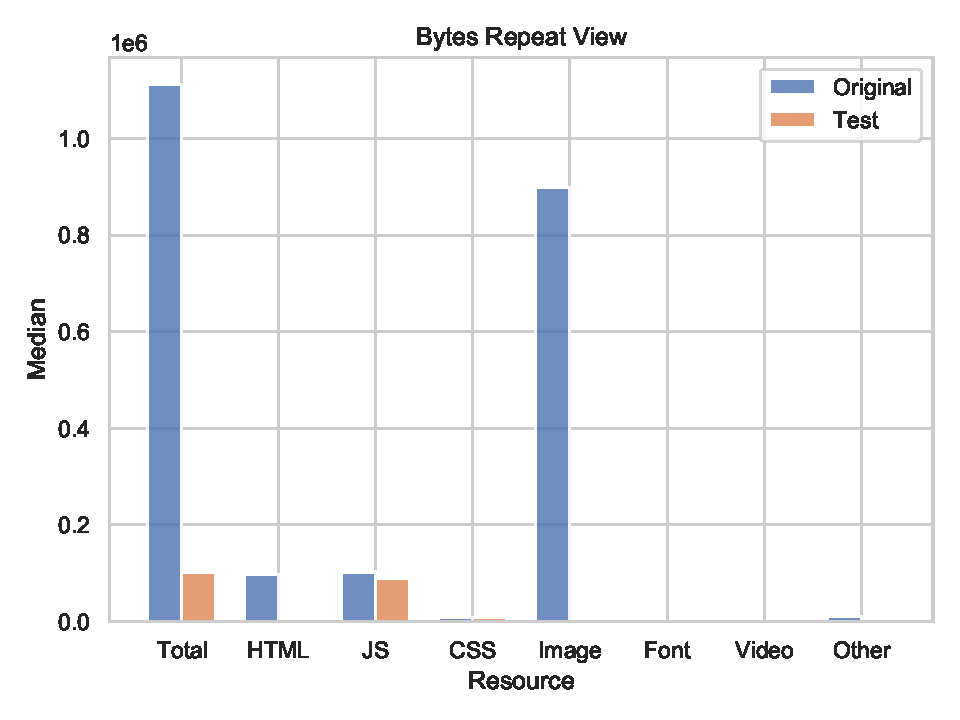
\includegraphics[width=1\linewidth]{plots/original_vs_test/bytes_rv.pdf}
		%\caption{Bytes First View}
		\label{fig:sub1}
	\end{subfigure}%
	\begin{subfigure}{.5\textwidth}
		\centering
		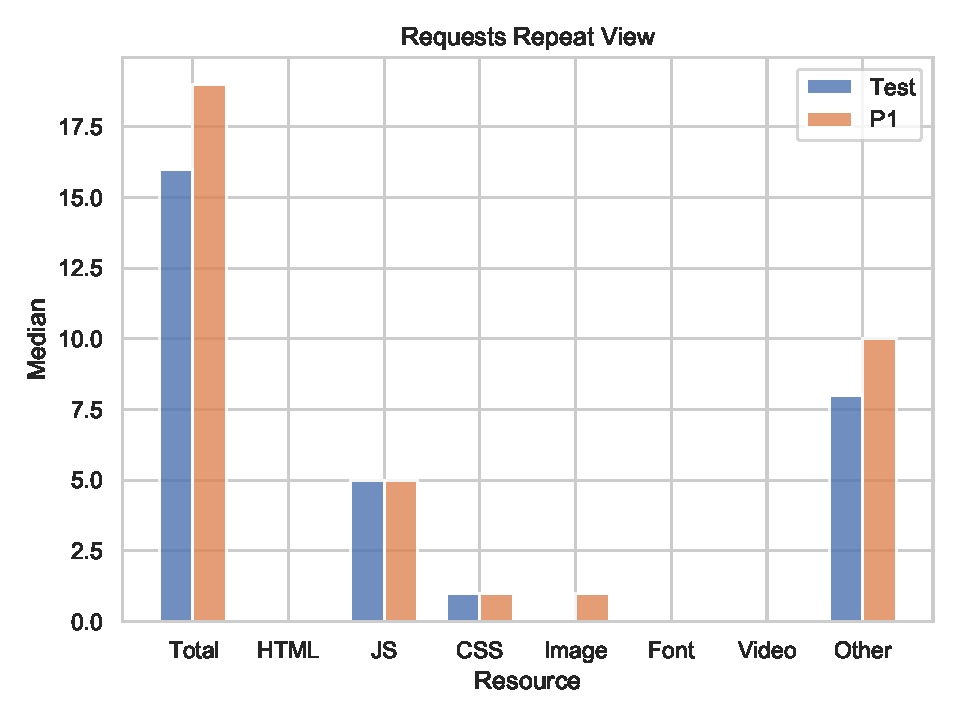
\includegraphics[width=1\linewidth]{plots/original_vs_test/requests_rv.pdf}
		%\caption{Requests}
		\label{fig:sub2}
	\end{subfigure}
	\caption{Page Weight Repeat View, Original vs Test.}
	\label{figure:plt_original_test}
\end{figure}


% --- PLT ---
\begin{figure}
	\centering
	\begin{subfigure}{.5\textwidth}
		\centering
		\includegraphics[width=1\linewidth]{plots/original_vs_test/plt_fv.pdf}
		%\caption{A subfigure}
		\label{fig:sub1}
	\end{subfigure}%
	\begin{subfigure}{.5\textwidth}
		\centering
		\includegraphics[width=1\linewidth]{plots/original_vs_test/plt_rv.pdf}
		%\caption{A subfigure}
		\label{fig:sub2}
	\end{subfigure}
	\caption{Page Load Time, Original vs Test.}
	\label{figure:plt_original_test}
\end{figure}


% --- FCP ---
\begin{figure}
	\centering
	\begin{subfigure}{.5\textwidth}
		\centering
		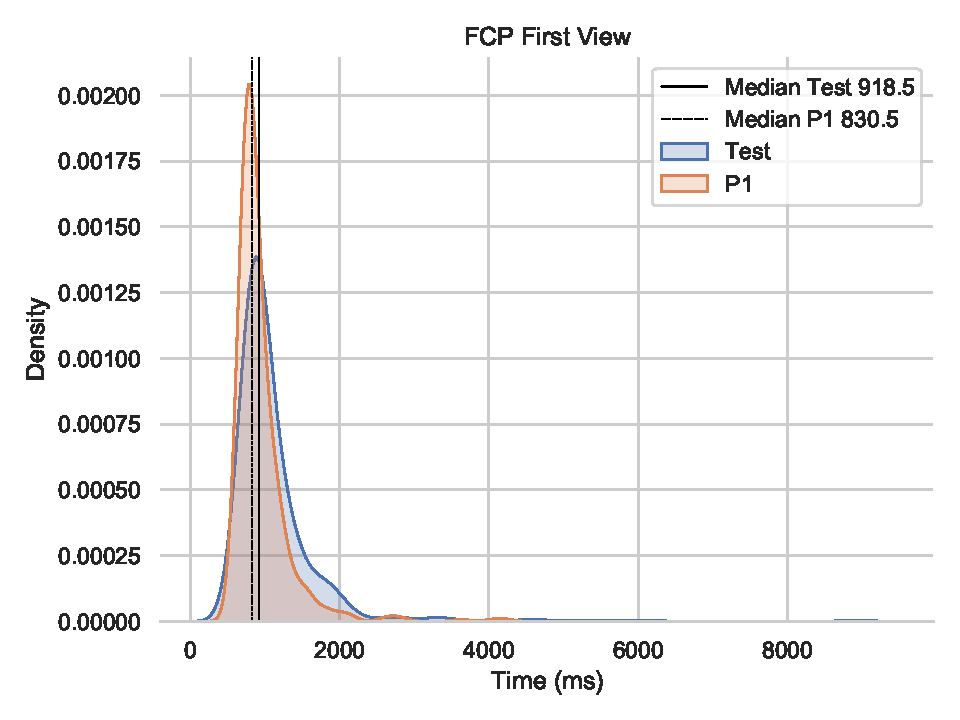
\includegraphics[width=1\linewidth]{plots/original_vs_test/fcp_fv.pdf}
		%\caption{A subfigure}
		\label{fig:sub1}
	\end{subfigure}%
	\begin{subfigure}{.5\textwidth}
		\centering
		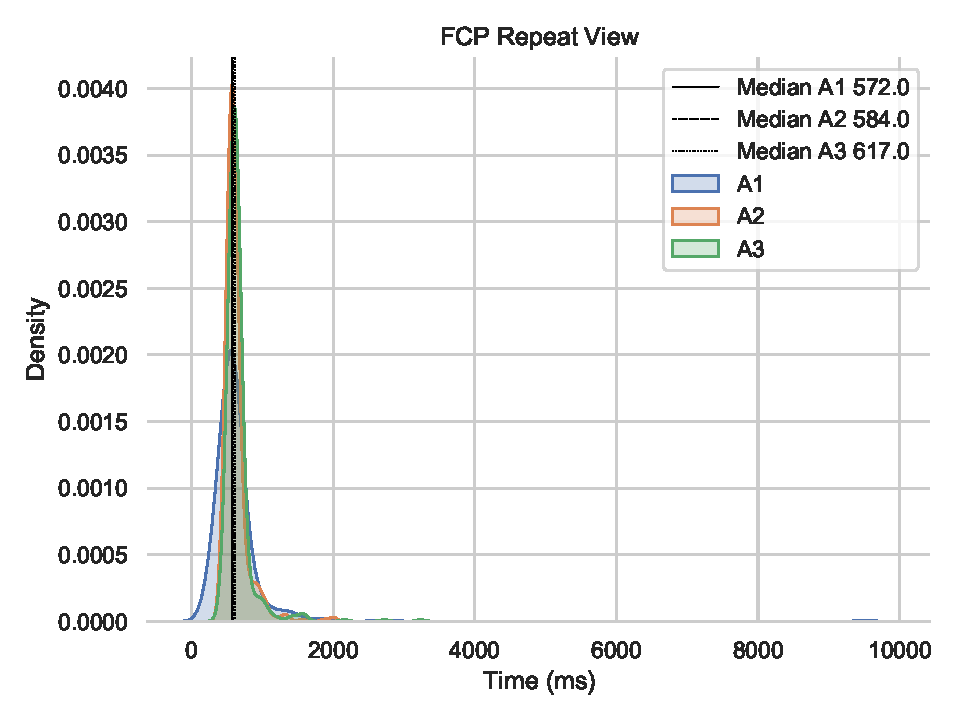
\includegraphics[width=1\linewidth]{plots/original_vs_test/fcp_rv.pdf}
		%\caption{A subfigure}
		\label{fig:sub2}
	\end{subfigure}
	\caption{First Contentful Paint, Original vs Test.}
	\label{figure:fcp_original_test}
\end{figure}

% add LCP / Speed Index ?

\clearpage


% -------------------------------------------------------------

\subsection{Test Website without GA vs Variant P1}

This section compares the test website which does not include any tracking script, and the variant P1 where the GA tracking script is included at top of the head section in the main html document. 
Hence, the only difference between the two websites is the tracking script, which is represented in the diagrams.

% [Page Weight]

The bytes in the page weight in the first view is identical, only that more bytes for JS are downloaded.
Those bytes are the tracking script.
For the requests, apart from more requests for JS, also more images and other resources are requested in the variant P1 and it can be assumed that those requests are trigged by the tracking script.

%figure X


% [PLT, LCP]

The values for the PLT, the metric which represents how long the navigation process takes place, are very similar for both versions, for the first and also repeat view.
Same goes for the visual metric LCP, which is nearly identical for both versions.

%figure X

% [Conclusion]

It can be concluded the adding the tracking script has nearly no effect on web performance.
Although the page weight gets slightly bigger with the tracking script included, this weight has no negative impact on the page load time nor user-centric performance metrics such as LCP.


% --- Page Weight FV ---
\begin{figure}
	\centering
	\begin{subfigure}{.5\textwidth}
		\centering
		\includegraphics[width=1\linewidth]{plots/test_vs_position/bytes_fv.pdf}
		\caption{Bytes First View}
		\label{fig:sub1}
	\end{subfigure}%
	\begin{subfigure}{.5\textwidth}
		\centering
		\includegraphics[width=1\linewidth]{plots/test_vs_position/requests_fv.pdf}
		\caption{Requests First View}
		\label{fig:sub2}
	\end{subfigure}
	\caption{Page Weight First View, Test vs Variant P1.}
	\label{figure:plt_original_test}
\end{figure}


% --- PLT ---
\begin{figure}
	\centering
	\begin{subfigure}{.5\textwidth}
		\centering
		\includegraphics[width=1\linewidth]{plots/test_vs_position/plt_fv.pdf}
		%\caption{A subfigure}
		\label{fig:sub1}
	\end{subfigure}%
	\begin{subfigure}{.5\textwidth}
		\centering
		\includegraphics[width=1\linewidth]{plots/test_vs_position/plt_rv.pdf}
		%\caption{A subfigure}
		\label{fig:sub2}
	\end{subfigure}
	\caption{Page Load Time, Test vs Variant P1.}
	\label{figure:plt_original_test}
\end{figure}


% --- LCP ---
\begin{figure}
	\centering
	\begin{subfigure}{.5\textwidth}
		\centering
		\includegraphics[width=1\linewidth]{plots/test_vs_position/lcp_fv.pdf}
		%\caption{A subfigure}
		\label{fig:sub1}
	\end{subfigure}%
	\begin{subfigure}{.5\textwidth}
		\centering
		\includegraphics[width=1\linewidth]{plots/test_vs_position/lcp_rv.pdf}
		%\caption{A subfigure}
		\label{fig:sub2}
	\end{subfigure}
	\caption{Largest Contentful Paint, Test vs Variant P1.}
	\label{figure:plt_original_test}
\end{figure}


\clearpage


% -------------------------------------------------------------

\subsection{IV Position: Variant P1 vs Variant P2 vs Variant P3}


The first independent variable.. 
% whats the impact of the position ?

%TTFB: - Repeat View is slower (on median) ??


DOM Content Loaded: ...

PLT: ...

Speed Index: ...

LCP: ...

% --- DCL ---
\begin{figure}
	\centering
	\begin{subfigure}{.5\textwidth}
		\centering
		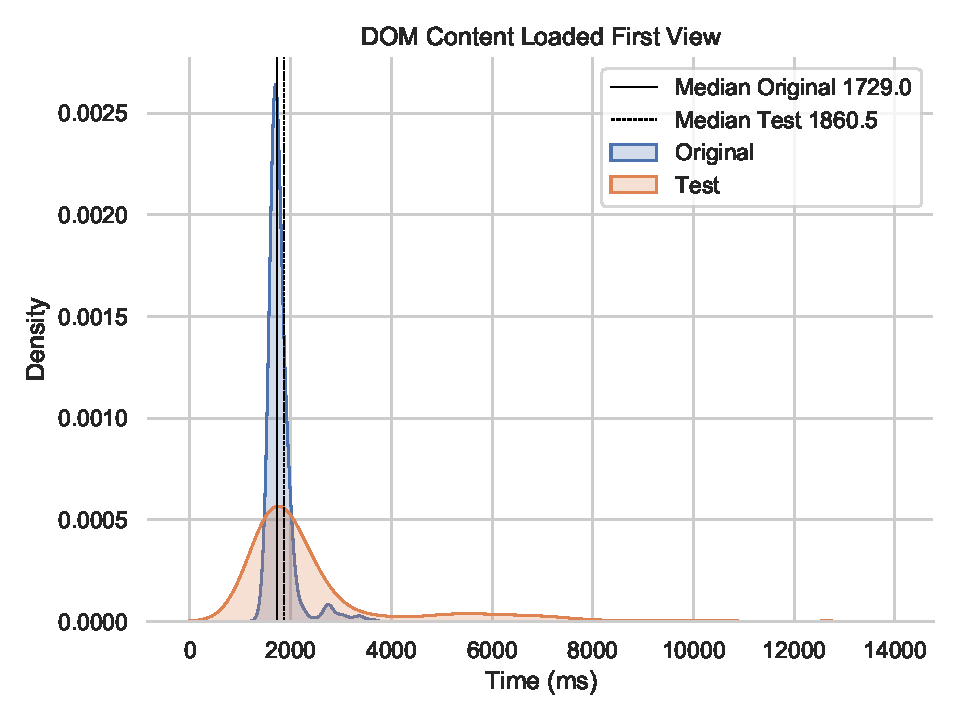
\includegraphics[width=1\linewidth]{plots/IV1_position/dcl_fv.pdf}
		%\caption{A subfigure}
		\label{fig:sub1}
	\end{subfigure}%
	\begin{subfigure}{.5\textwidth}
		\centering
		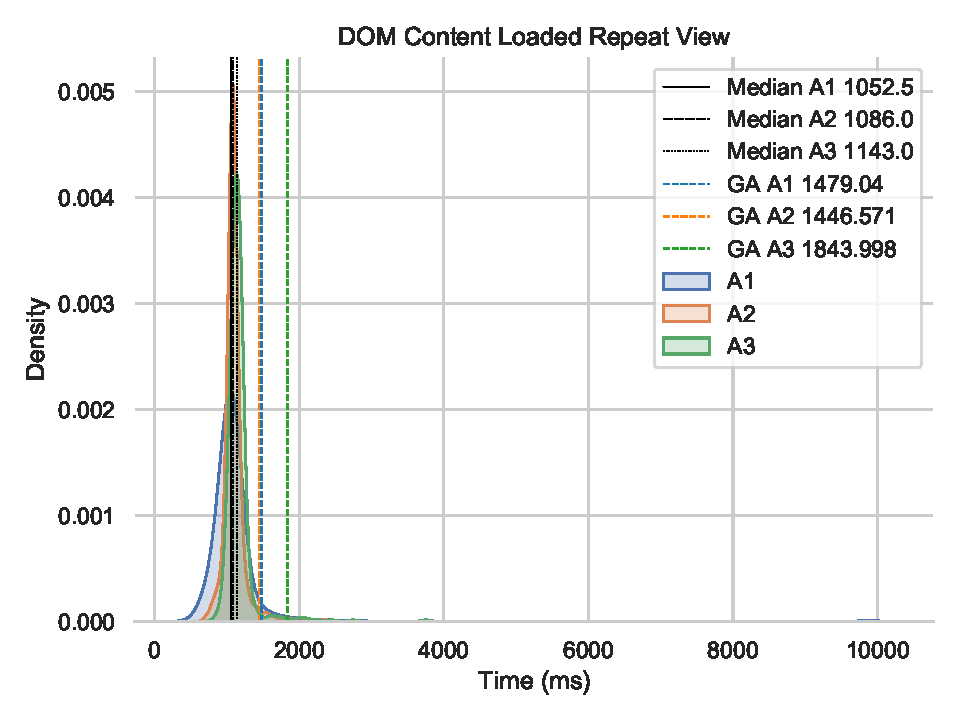
\includegraphics[width=1\linewidth]{plots/IV1_position/dcl_rv.pdf}
		%\caption{A subfigure}
		\label{fig:sub2}
	\end{subfigure}
	\caption{DOM Content Loaded, Variant P1 vs Variant P2 vs Variant P3, with GA.}
	\label{figure:plt_original_test}
\end{figure}


% --- PLT ---
\begin{figure}
	\centering
	\begin{subfigure}{.5\textwidth}
		\centering
		\includegraphics[width=1\linewidth]{plots/IV1_position/plt_fv.pdf}
		%\caption{A subfigure}
		\label{fig:sub1}
	\end{subfigure}%
	\begin{subfigure}{.5\textwidth}
		\centering
		\includegraphics[width=1\linewidth]{plots/IV1_position/plt_rv.pdf}
		%\caption{A subfigure}
		\label{fig:sub2}
	\end{subfigure}
	\caption{Page Load Time, Variant P1 vs Variant P2 vs Variant P3, with GA.}
	\label{figure:plt_original_test}
\end{figure}


% --- SI ---
\begin{figure}
	\centering
	\begin{subfigure}{.5\textwidth}
		\centering
		\includegraphics[width=1\linewidth]{plots/IV1_position/si_fv.pdf}
		%\caption{A subfigure}
		\label{fig:sub1}
	\end{subfigure}%
	\begin{subfigure}{.5\textwidth}
		\centering
		\includegraphics[width=1\linewidth]{plots/IV1_position/si_rv.pdf}
		%\caption{A subfigure}
		\label{fig:sub2}
	\end{subfigure}
	\caption{Speed Index, Variant P1 vs Variant P2 vs Variant P3.}
	\label{figure:plt_original_test}
\end{figure}


% --- LCP ---
\begin{figure}
	\centering
	\begin{subfigure}{.5\textwidth}
		\centering
		\includegraphics[width=1\linewidth]{plots/IV1_position/lcp_fv.pdf}
		%\caption{A subfigure}
		\label{fig:sub1}
	\end{subfigure}%
	\begin{subfigure}{.5\textwidth}
		\centering
		\includegraphics[width=1\linewidth]{plots/IV1_position/lcp_rv.pdf}
		%\caption{A subfigure}
		\label{fig:sub2}
	\end{subfigure}
	\caption{Largest Contentful Paint, Variant P1 vs Variant P2 vs Variant P3.}
	\label{figure:plt_original_test}
\end{figure}


\clearpage



% -------------------------------------------------------------


\subsection{IV Attribute: Variant A1 vs Variant A2 vs Variant A3}

% so does it really not matter ?

%The GA measurements are median over all views, first view and repeat view.
%Hence they are always the same for FV and RV.
%With this setup, we do not have different data for RUM measurements from Google depending on if the website was loaded the first time or from cache.


PLT: ...

Fully Loaded: ...

Speed Index: ...

LCP: ...


%CLS: medians are all the same ??

% --- PLT ---
\begin{figure}
	\centering
	\begin{subfigure}{.5\textwidth}
		\centering
		\includegraphics[width=1\linewidth]{plots/IV2_attribute/plt_fv.pdf}
		%\caption{A subfigure}
		\label{fig:sub1}
	\end{subfigure}%
	\begin{subfigure}{.5\textwidth}
		\centering
		\includegraphics[width=1\linewidth]{plots/IV2_attribute/plt_rv.pdf}
		%\caption{A subfigure}
		\label{fig:sub2}
	\end{subfigure}
	\caption{Page Load Time, Variant A1 vs Variant A2 vs Variant A3, with GA.}
	\label{figure:plt_original_test}
\end{figure}


% --- Fully Loaded ---
\begin{figure}
	\centering
	\begin{subfigure}{.5\textwidth}
		\centering
		\includegraphics[width=1\linewidth]{plots/IV2_attribute/fully_loaded_fv.pdf}
		%\caption{A subfigure}
		\label{fig:sub1}
	\end{subfigure}%
	\begin{subfigure}{.5\textwidth}
		\centering
		\includegraphics[width=1\linewidth]{plots/IV2_attribute/fully_loaded_rv.pdf}
		%\caption{A subfigure}
		\label{fig:sub2}
	\end{subfigure}
	\caption{Fully Loaded, Variant A1 vs Variant A2 vs Variant A3.}
	\label{figure:plt_original_test}
\end{figure}

% FV: A1 seems to have less distribution, where as A2 and A3 have some distributed data


% --- SI ---
\begin{figure}
	\centering
	\begin{subfigure}{.5\textwidth}
		\centering
		\includegraphics[width=1\linewidth]{plots/IV2_attribute/si_fv.pdf}
		%\caption{A subfigure}
		\label{fig:sub1}
	\end{subfigure}%
	\begin{subfigure}{.5\textwidth}
		\centering
		\includegraphics[width=1\linewidth]{plots/IV2_attribute/si_rv.pdf}
		%\caption{A subfigure}
		\label{fig:sub2}
	\end{subfigure}
	\caption{Speed Index, Variant A1 vs Variant A2 vs Variant A3.}
	\label{figure:plt_original_test}
\end{figure}

% --- LCP ---
\begin{figure}
	\centering
	\begin{subfigure}{.5\textwidth}
		\centering
		\includegraphics[width=1\linewidth]{plots/IV2_attribute/lcp_fv.pdf}
		%\caption{A subfigure}
		\label{fig:sub1}
	\end{subfigure}%
	\begin{subfigure}{.5\textwidth}
		\centering
		\includegraphics[width=1\linewidth]{plots/IV2_attribute/lcp_rv.pdf}
		%\caption{A subfigure}
		\label{fig:sub2}
	\end{subfigure}
	\caption{Largest Contentful Paint, Variant A1 vs Variant A2 vs Variant A3.}
	\label{figure:plt_original_test}
\end{figure}



\clearpage



% -------------------------------------------------------------

\subsection{IV Other Script: Variant OS1 vs Variant OS2}

% only IV OS seems to have some impact on the performance of the website
% This makes sense as an additional resource has to be loaded.
% The IVs Position and Attribute only alter how the resource is being loaded, but they dont change the page weight



PLT: ...

Fully Loaded: ...

Speed Index: ...

Total Blocking Time: ...


% --- PLT ---
\begin{figure}
	\centering
	\begin{subfigure}{.5\textwidth}
		\centering
		\includegraphics[width=1\linewidth]{plots/IV3_other_script/plt_fv.pdf}
		%\caption{A subfigure}
		\label{fig:sub1}
	\end{subfigure}%
	\begin{subfigure}{.5\textwidth}
		\centering
		\includegraphics[width=1\linewidth]{plots/IV3_other_script/plt_rv.pdf}
		%\caption{A subfigure}
		\label{fig:sub2}
	\end{subfigure}
	\caption{Page Load Time, Variant OS1 vs Variant OS2, with GA.}
	\label{figure:plt_original_test}
\end{figure}


% --- Fully Loaded ---
\begin{figure}
	\centering
	\begin{subfigure}{.5\textwidth}
		\centering
		\includegraphics[width=1\linewidth]{plots/IV3_other_script/fully_loaded_fv.pdf}
		%\caption{A subfigure}
		\label{fig:sub1}
	\end{subfigure}%
	\begin{subfigure}{.5\textwidth}
		\centering
		\includegraphics[width=1\linewidth]{plots/IV3_other_script/fully_loaded_rv.pdf}
		%\caption{A subfigure}
		\label{fig:sub2}
	\end{subfigure}
	\caption{Fully Loaded, Variant OS1 vs Variant OS2.}
	\label{figure:plt_original_test}
\end{figure}


% --- SI ---
\begin{figure}
	\centering
	\begin{subfigure}{.5\textwidth}
		\centering
		\includegraphics[width=1\linewidth]{plots/IV3_other_script/si_fv.pdf}
		%\caption{A subfigure}
		\label{fig:sub1}
	\end{subfigure}%
	\begin{subfigure}{.5\textwidth}
		\centering
		\includegraphics[width=1\linewidth]{plots/IV3_other_script/si_rv.pdf}
		%\caption{A subfigure}
		\label{fig:sub2}
	\end{subfigure}
	\caption{Speed Index, Variant OS1 vs Variant OS2.}
	\label{figure:plt_original_test}
\end{figure}


% --- TBT ---
\begin{figure}
	\centering
	\begin{subfigure}{.5\textwidth}
		\centering
		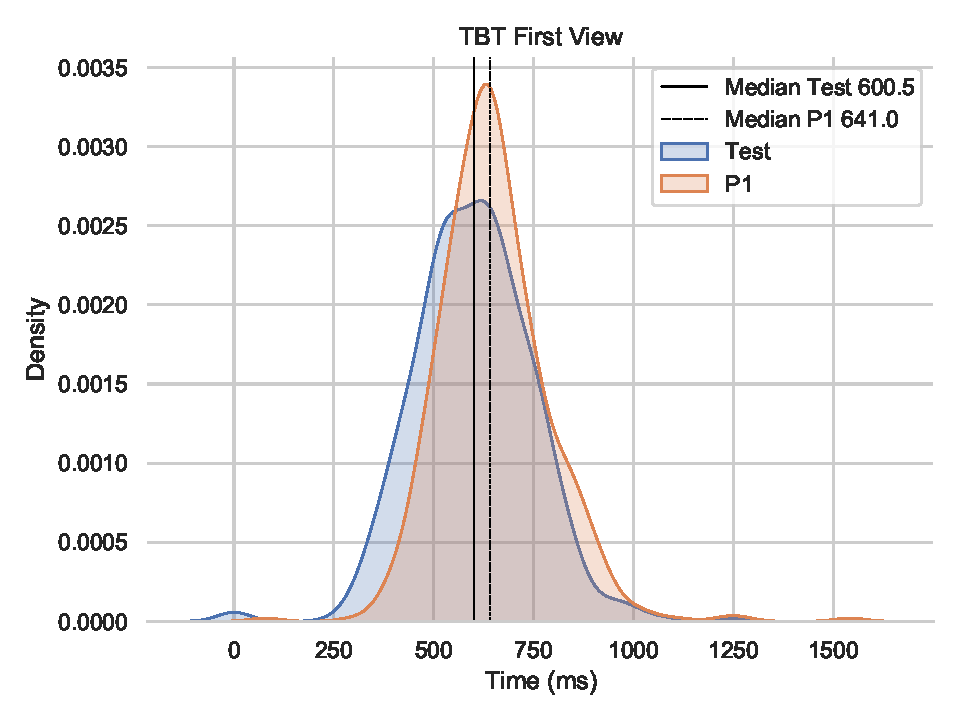
\includegraphics[width=1\linewidth]{plots/IV3_other_script/tbt_fv.pdf}
		%\caption{A subfigure}
		\label{fig:sub1}
	\end{subfigure}%
	\begin{subfigure}{.5\textwidth}
		\centering
		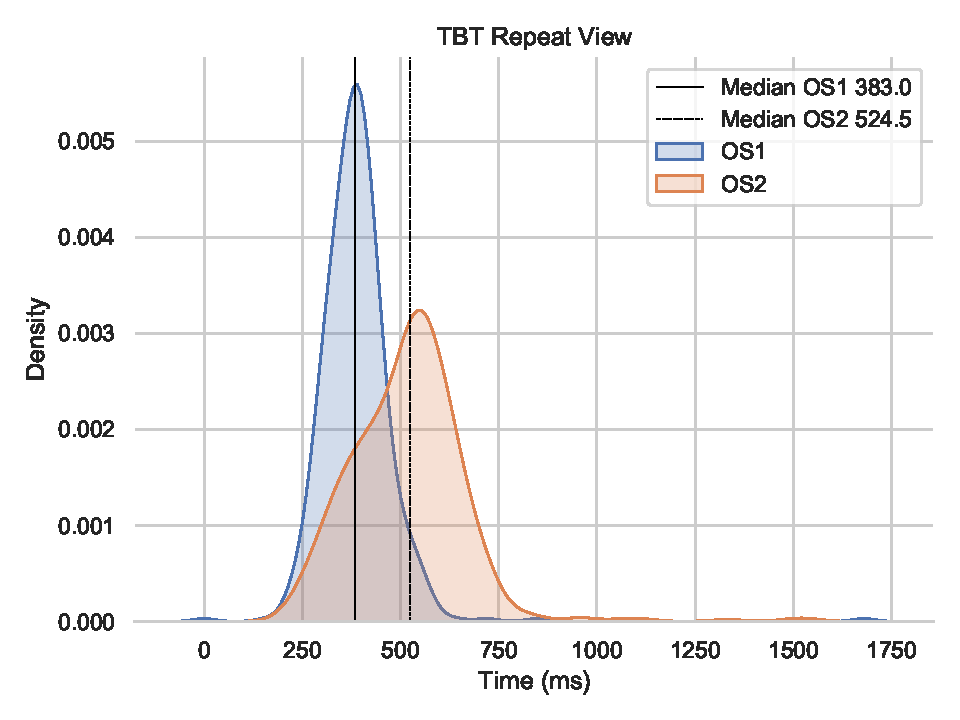
\includegraphics[width=1\linewidth]{plots/IV3_other_script/tbt_rv.pdf}
		%\caption{A subfigure}
		\label{fig:sub2}
	\end{subfigure}
	\caption{Total Blocking Time, Variant OS1 vs Variant OS2.}
	\label{figure:plt_original_test}
\end{figure}

\clearpage


% ----------------------------------------------------------------------------------------------------


\section{Other Aspects and Points of Discussion}

% Quality of the collected data.
% this is part of research question: do the different variants change the collected data ?


% For each attempt, describe: Threats to validity, generalizability


% -------------------------------------------------------------

\subsection{Generalizability}

% meine Daten zeige nur für Chrome, MacBook, diese Geschwindigkeit etc.
% Und auch nur für diese Test-Website
% Die Schwierigkeit der Generalisierbarkeit ist eines der grössten Probleme bei dieser Fragestellung




% -------------------------------------------------------------



\subsection{Internal and External Validity}



% The quality and quantity of the data needs to be discussed
% Quality: There are chances that some data are malformed, e.g. because internet connection was bad, etc.
% Quantity: Is the amount of data sufficient to make the evaluation generalisable



% 2016 Kohavi: Analysis of Experiments
















% ----------- To big to fail... to delete :/ -----------


% \subsection{Bulk Test Overview: Description of test result page}

% \begin{itemize}
% \item Each test has Test ID: YYMMDD\textunderscore random\textunderscore random
% \item Test results after bulk test available under \url{http://localhost:4000/result/{testID}/}
% \item For each test run, following data is available:
% 	\begin{itemize}
% 	\item Link to test results: Test result page as same as for single test run
% 	\item Median load time (First view)
% 	\item Median load time (Repeat view)
% 	\item Median Speed Index (First View)
% 	\item Raw page data (file: [TestID\textunderscore summary.csv]
% 	\item Raw object data (file: [TestID\textunderscore details.csv])
% 	\item Http archive (.har) (file: json)
% 	\end{itemize}
	
% \item Average First View Load Time
% \item Average Repeat View Load Time
% \item Combined Raw: Page Data  (file: [TestID\textunderscore summary.csv])
% \item Combined Raw: Object Data (file: [TestID\textunderscore details.csv]). For 100 test runs, this file is appr. 20 MB, 24432 rows, 76 columns. 
% \item Aggregate Statistics (file: [TestID\textunderscore aggregate.csv])
% \end{itemize}




% \subsection{Compare Section}

% WPT has a feature to compare multiple tests.
% Accessible under compare URL: \url{http://localhost:4000/video/compare.php?tests={TestID},{TestID},...}

% The compare page contains:

% \begin{itemize}
% \item Film strip
% \item Waterfall diagram
% \item Visual Progress diagram
% \item Timings diagram:
% 	\begin{itemize}
% 	\item Visually Complete (First View Visually Complete Median)
% 	\item Last Visual Change
% 	\item Load Time (onload)
% 	\item ...
% 	\end{itemize}
% \item Cumulative Layout Shift diagram
% \item Requests diagram
% \item Bytes diagram
% \item Visually complete
% \item Last Visual Change
% \item Load Time (onload)
% \item Load Time (Fully Loaded)
% \item DOM Content Loaded
% \item Speed Index
% \item Time to First Byte
% \item Time to Title
% \item Time to Start Render
% \item CPU Busy Time
% \item 85\% Visually Complete
% \item 90\% Visually Complete
% \item 95\% Visually Complete
% \item 99\% Visually Complete
% \item First Contentful Paint
% \item First Meaningful Paint
% \item Largest Contenful Paint
% \item Cumulative Layout Shift
% \item html Requests
% \item html Bytes
% \item js Requests
% \item js Bytes
% \item css Requests
% \item css Bytes
% \item image Requests
% \item image Bytes
% \item flash Requests
% \item flash Bytes
% \item font Requests
% \item font Bytes
% \item video Requests
% \item video Bytes
% \item other Requests
% \item other Bytes
% \end{itemize}




